\documentclass[conference]{IEEEtran}
\IEEEoverridecommandlockouts
\usepackage{stfloats} %针对双栏图 实现h t b p
\usepackage{makecell} %表格中一个单元格的文字换行
\usepackage{threeparttable} %表格注解
\usepackage{enumitem}  % item缩进
\usepackage{array}   % 表格内文字居中
\usepackage{booktabs}
%%%%%%%%%%%%%%%%%%%%%%%%%%%%%%%%%%%%%%%%%%%%%%%%%%%%%%%%%
%    Comments
%%%%%%%%%%%%%%%%%%%%%%%%%%%%%%%%%%%%%%%%%%%%%%%%%%%%%%%%%
\usepackage{verbatim}
%%%%%%%%%%%%%%%%%%%%%%%%%%%%%%%%%%%%%%%%%%%%%%%%%%%%%%%%%
%\usepackage[varg]{txfonts}
\usepackage{float}
\usepackage{bm}
\usepackage{eqparbox}
\usepackage{booktabs}
\usepackage{stmaryrd}
\usepackage{amssymb}
\usepackage{mathrsfs}
\usepackage{epsfig,graphics}
\usepackage{amsmath}
\usepackage{wasysym}
\usepackage{graphicx}
\usepackage{tabularx}
\usepackage{url}

%\usepackage{algpseudocode}
%\usepackage{appendix}

\usepackage{pgfplots}
\usepackage{pgfplotstable}
\usepackage{pgfplots} % used for showing all the figure
\pgfplotsset{
	compat=1.5
}

%\usepackage{cite}
\usepackage{amsfonts}

%�㷨����
\usepackage{algorithm}
%\usepackage[ruled]{algorithm2e}
\usepackage{algorithmicx}
\usepackage{algpseudocode}  %����
\usepackage{textcomp}  %����\textacutedbl �İ�,���׵�����
%\usepackage{authblk} %���߷�ʽ�� ��Ҫ�õİ���
\usepackage{xcolor}
%����ĺϲ� �кϲ�
\usepackage{multirow}
%������Ҽӵ�����ע�͵�
%\usepackage{comment}


\def\BibTeX{{\rm B\kern-.05em{\sc i\kern-.025em b}\kern-.08em
    T\kern-.1667em\lower.7ex\hbox{E}\kern-.125emX}}


\usepgfplotslibrary{groupplots}
%\usepackage[ngerman]{babel}
%%%%%%%%%%%%%%%%%%%%%%%%%%%%%%%%%%%%%%%%%%%%%%%%%%%%%%%%%
%    Algorithm
%%%%%%%%%%%%%%%%%%%%%%%%%%%%%%%%%%%%%%%%%%%%%%%%%%%%%%%%%
%\usepackage[]{algorithm2e}
%\usepackage{algorithmic}
\usepackage{algorithm}
\usepackage{multicol}
\usepackage{algpseudocode}
%%%%%%%%%%%%%%%%%%%%%%%%%%%%%%%%%%%%%%%%%%%%%%%%%%%%%%%%%


\newcommand{\Real}{{\mathbb R}}
\newcommand{\Inh}[2]{\mathsf{Inh}\mathsf{(#1, #2)}}
\newcommand{\Cal}[2]{\mathsf{Cal}\mathsf{(#1, #2)}}
\newcommand{\Con}[2]{\mathsf{Con}\mathsf{(#1, #2)}}
\newcommand{\Cre}[2]{\mathsf{Cre}\mathsf{(#1, #2)}}
\newcommand{\Ref}[2]{\mathsf{Ref}\mathsf{(#1, #2)}}
\newcommand{\rand}{\wedge}
\newcommand{\ror}{\vee}
\newcommand{\rimply}{\Rightarrow}
\newcommand{\rr}{\rightarrow}
\newcommand{\nr}{\rightsquigarrow}
\newcommand{\rnot}{!}
\newcommand{\Instances}[1]{\mathsf{Inst}\mathsf{(#1)}}
\newcommand{\TypeOf}[1]{\mathsf{Type}\mathsf{(#1)}}
\newcommand{\AttrValue}[2]{\mathsf{AttrVal}\mathsf{(#1, #2)}}
\newcommand{\Value}[1]{\mathsf{Val}\mathsf{(#1)}}
\newcommand{\InitialValue}[1]{\mathsf{InitVal}\mathsf{(#1)}}
\newcommand{\Contains}[2]{\mathsf{Con}\mathsf{(#1, #2)}}
\newcommand{\patomic}{\mathsf{atomic}}
\newcommand{\pskip}{\mathsf{skip}}
\newcommand{\pmf}[1]{\mathsf{#1}}
\newcommand{\szihao}{\fontsize{1pt}{1pt}\selectfont}
\newcommand{\sfrac}{\szihao \dfrac}
\newcommand{\WI}[1]{\texttt{#1}}
\newcommand{\cname}[1]{{\small ${#1}$}}
%\newcommand{\tabincell}[2]{\begin{tabular}{@{}#1@{}}#2\end{tabular}}
\renewcommand{\algorithmicrequire}{\textbf{Input:}}  % Use Input in the format of Algorithm
\renewcommand{\algorithmicensure}{\textbf{Output:}} % Use Output in the format of Algorithm


% correct bad hyphenation here
\hyphenation{op-tical net-works semi-conduc-tor}
\usepackage[square, comma, sort&compress, numbers]{natbib}
\usepackage{color}
\definecolor{gray}{rgb}{0.4,0.4,0.4}
\definecolor{darkblue}{rgb}{0.0,0.0,0.6}
\definecolor{cyan}{rgb}{0.0,0.6,0.6}
\usepackage{epstopdf}

\usepackage[colorlinks,
            linkcolor=black,
            anchorcolor=black,
            citecolor=blue,
			urlcolor=black,
            bookmarks=true
            ]{hyperref}


\newcommand{\TODO}[2]{{\textcolor{blue}{#1}}$\to${\textcolor{red}{#2}}}
\newcommand{\SOLVED}[2]{#2}
\newcommand{\HIGHLIGHT}[1]{{\textcolor{red}{#1}}}



%%%%%%%%%%%%%%%%%%%%%%%%%%%%%%%%%%%%%%%%%%%%%%%%%%%%%%%%%%%%%%%%%
\newcommand{\lds}[4]{
$\bb{#1}\sfbe{
	#2
}~=~
	\lambda #3.
(
	#4
)$}



\newcommand{\sfbe}[1]{\llbracket~#1~\rrbracket}

\newcommand{\denotationalsemantics}[4]{
{\footnotesize$
\bb{#1}\llbracket
	#2
\rrbracket=~\{
	#3
		~\mid~
	#4
\}$}}
\newcommand{\ins}[1]{$\lfloor$#1$\rceil$}
\newcommand{\lr}{\longrightarrow}
\newcommand{\bb}[1]{{\mathbb{#1}}}
\newcommand{\sfb}[1]{\textlbrackdbl~#1~\textrbrackdbl}
\newcommand{\la}{\langle}

\newcommand{\ra}{\rangle}
\newcommand{\nit}{\noindent}
\newcommand{\fbv}{formula_{bv}}
\newcommand{\s}{\sigma}
\newcommand{\sip}{\sigma^\prime}

%%%%%%%%%%%%%%%%%%%%%%%%%%%%%%%%%%%%%%
\newcommand{\code}[1]{{\texttt{#1}}}
\newcommand{\address}[1]{{\textcolor{gray}{\texttt{#1}}}}
\newcommand{\haddress}[1]{{\textcolor{blue}{\texttt{#1}}}}
\newcommand{\hcode}[1]{{\textcolor{blue}{\texttt{#1}}}} 

\begin{document}

\title{SAGANFuzzer: A Deep Adversarial Networks based Industrial Control Protocol Fuzzing Framework from a Self-Attention Perspective \\}
%\author{ %Anonymous
\IEEEauthorblockN{
Zhihui Li\IEEEauthorrefmark{2},
Jiawen Xiong\IEEEauthorrefmark{2},
%Hui Zhao\IEEEauthorrefmark{1},
Jianqi Shi\IEEEauthorrefmark{2} and
Yanhong Huang\IEEEauthorrefmark{2}\IEEEauthorrefmark{3}
}
%\IEEEauthorblockA{\IEEEauthorrefmark{1}National Trusted Embedded Software Engineering Technology Research Center\\
%East China Normal University, Shanghai, China\\
%}
\IEEEauthorblockA{\IEEEauthorrefmark{3}Hardware/Software Co-Design Technology and Application Engineering Research Center, Shanghai, China\\
}
\IEEEauthorblockA{\IEEEauthorrefmark{2}Shanghai Key Laboratory of Trustworthy Computing, East China Normal University, Shanghai, China\\
Email:\{zhihui.li, jiawen.xiong\}@ntesec.ecnu.edu.cn}
%Email:\{zhihui.li, hui.zhao, jianqi.shi, yanhong.huang, jiawen.xiong \}@ntesec.ecnu.edu.cn}
} 
\author{Wanyou Lv$^{1}$ \and
	Bohao Wang$^{2}$ \and
	Zhihui Li$^{3}$ \and
	Jianqi Shi$^{3,*}$ \and
	Yanhong Huang$^{4}$
}

%\authorrunning{Short form of author list} % if too long for running head


%\date{Received: date / Accepted: date}
\date{2020/04/07}
% The correct dates will be entered by the editor

% Comment for arXiv
%\titlerunning{Journal of Intelligent Manufacturing}
%\authorrunning{Journal of Intelligent Manufacturing}

%\titlerunning{

\maketitle

\begin{abstract}
The Industrial Control Protocol (ICP) is the cornerstone of the communication of the Industrial Control System (ICS).
%, and its importance to the ICS is self-evident. 
If the security of ICPs can be guaranteed, the security of ICSs can be guaranteed to a large extent. However, due to the strong diversity of the industrial control environment applicable to ICPs which causes the meaning of the same parameter in different applications varies greatly, it is difficult for testers to formulate a series of universal security rules. Therefore, fuzz testing (fuzzing) has already become the main method of detecting vulnerabilities in ICPs. However, the process of fuzzing relies heavily on the specification of ICPs. And it will take a lot of time and manual engineering to analyze and understand the specification. In this paper, we proposed a new simple and smart sequence generation neural network framework based on Improved Self-Attention Generative Adversarial Networks (SAGAN), called SAGANFuzzer, to solve the problems. Moreover, we put forward a series of performance metrics in the field of fuzzing to evaluate different models. Compared with traditional methods, our framework can generate massive fake but plausible test protocol message automatically in a short time without protocol specification; compared with other deep learning works for fuzzing, our framework can not only test multi-dimensional input effectively but also increase the probability of vulnerabilities being triggered while being more parallelizable and requiring significantly less time to train. We evaluate its performance by testing several typical ICPs, including MQTT and Modbus. Extensive experiments demonstrate significant improvements over test effectiveness and efficiency: the accuracy of correctly generating test case packages is 86.08\% and 92.71\% in different data scales, the F-measure reaches 82.08\% and 85.02\%, and the test effectiveness and efficiency are 8.03\% and 5.26\% higher than the WGAN-based model.

%correctly generates the format and message content of the test case package. 其准确率分别为86.08%、92.71%,,F-measure分别达到了82.08%和85.02%,测试有效性和效率比WGAN-based model分别高了8.03%,5.26%。   
%\textcolor[rgb]{1,0,0}{\#\#\#\#\#\#\#\#  Here can specify specific values.}
\end{abstract}

\begin{IEEEkeywords}
deep adversarial learning, self-attention, convolution neural networks, fuzz testing, industrial control protocol
\end{IEEEkeywords}

\section{Introduction}
Industry 4.0 and Smart Manufacturing as a national plan for many countries are promoting a new round of industrial prosperity globally. In manufacturing, there are many safety-critical control systems, and ensuring its safety (Based on IEC  61508 \cite{bell2006introduction}) and security (Based on IEC 62442 \cite{piggin2013development}) has been an important issue in academic and industry group. The entire system’s safety and security can be considered in many ways. Some perform formal verification \cite{braibant2011coquet} of embedded programs in the system. Others perform penetration testing \cite{mcdermott2001attack} to find system vulnerabilities. These efforts indeed improved system safety and security. However, intelligent manufacturing requires the increasing interconnectivity of ICSs. This reality exposes ICSs to more diverse and unexpected threats from outside, which has raised the potential risk to the security of ICSs.  ICPs, as the bridge of communication between various parts of ICSs, have promoted the construction of industry informatization and improved the production and management efficiency, but it also laid many potential risks for ICSs. With the inherent flaws of ICPs which are likely caused in the design and application phase and increasing frequency and sophistication of cyber-threats towards ICPs, it is urgent to take high-performance measures to mine vulnerabilities of ICPs.

A considerable part of attacks exploits the vulnerabilities of safety and security in ICPs. First, when these protocols are designed and applied in ICSs, there inevitably exist defects of design and differences between the implementation and the specifications. Some safety flaws were introduced at this time. Second, ICPs have common characteristics, such as real-time, functional code abuse and unencrypted, which can be exploited by malicious parties to launch attacks. Whether it is a safety flaw or a security flaw, we all need to find it out first, and then make up for it. Fuzzing \cite{miller1990empirical, miller1995fuzz} plays a vital role in finding these vulnerabilities. Its effectiveness has been proven by previous work \cite{wang2013design, voyiatzis2015modbus}. When performing the fuzz testing, we need to design and generate testing data according to the defined specifications, which brings some limitations. First, it does not work if it encounters an unknown specification. Second, the manual- based design for a specific protocol is not only demanding but time-consuming. Therefore, we attempt to find ways to improve the current situation. 

Benefiting from its recurrent structure, Long Short-Term Memory Network (LSTM) \cite{hochreiter1997long}, as an alternative type of neural network, shows great power in the precise timing of sequence data \cite{gers2002learning}. And Generative Adversarial Networks (GANs) \cite{goodfellow2014generative} is particularly famous for generating highly simulated images \cite{karras2018style}. Inspired by these, we attempted to integrate the characteristics of two networks to propose a combined model, replacing engineers, to generate massive fake but plausible test protocol messages. The model can not only be applied to both public and proprietary ICPs but also break the limitations above. In conclusion, we propose and design a fuzz testing methodology based on DCGAN (Deep Convolution Generative Adversarial Networks) \cite{radford2015unsupervised} in this study. The contributions are summarized as follows:


\begin{itemize}
\item[(1)] We propose a methodology based on Bi-directional LSTM (BLSTM) and DCGAN to deal with fuzzing data generation, in which it can intelligently learn to generate testing data by itself.
\item[(2)] On top of the approach, we build a universal fuzzing framework, the BLSTM-DCNNFuzz, which can deal with most ICPs’ fuzz testing. Also, in data processing, character- level data conversion is implemented.
\item[(3)] To evaluate its effectiveness, we apply it to fuzzing several ICPs. The results reveal that our method has good performance.
\end{itemize}

The remainder of this paper is organized as follows. Section \uppercase\expandafter{\romannumeral2} presents preliminary knowledge. Section \uppercase\expandafter{\romannumeral3} details optimized DCGAN algorithm and the entire methodology design. Section \uppercase\expandafter{\romannumeral4} presents the evaluation results. Section \uppercase\expandafter{\romannumeral5} discusses the related work. Section \uppercase\expandafter{\romannumeral6} concludes the paper and discusses some ideas about future work. 
%\section{Preliminary}
In this section, we introduce some preliminary knowledge. First, the basis of LSTM, GAN and DCGAN is presented.  We then introduce the preliminary knowledge of ICPs and their common features. Lastly, we give an overview of fuzz testing and its application in detecting ICPs' vulnerabilities.

\subsection{Long Short-Term memory}
Hochreiter and Schmidhuber (1997) first proposed LSTM to overcome the gradient vanishing problem of RNN (Recurrent Neural Networks). It is a special RNN that introduces an adaptive gating mechanism which can decides the degree to keep the previous state and avoid the problem of long-tern dependencies. Given a sequence $S = {{x_1}, {x_2}, …, {x_l}}$, where $l$ is the length of input text, LSTM processes it word by word. At time-step $t$, the memory $c_{t}$ and the hidden state $h_{t}$ are updated with the following equations:
\begin{equation}
\left[ \begin{array}{c}
\Gamma _u^{ < t > }\\
\Gamma _f^{ < t > }\\
\Gamma _o^{ < t > }\\
{{\hat c}_t}
\end{array} \right] = \left[ \begin{array}{c}
\sigma \\
\sigma \\
\sigma \\
\tanh 
\end{array} \right]W \cdot \left[ {{h_{t - 1}},{x_t}} \right]
\end{equation}
\begin{equation}
{c_t} = \Gamma _f^{ < t > } \odot {c_{t - 1}} + \Gamma _u^{ < t > } \odot {\hat c_t}
\end{equation}
\begin{equation}
{h_t} = \Gamma _o^{ < t > } \odot \tanh ({c_t})
\end{equation}
where $x_{t}$ is the input at the current time-step, $\Gamma _u$, $\Gamma _f$ and $\Gamma _o$ is the update gate activation, forget gate activation and output gate activation respectively, $\hat{c}$ is the current cell state, $\sigma$ denotes the logistic sigmoid function and $\odot$ denotes element-wise multiplication.

\subsection{Generative Adversarial Network}
Generative Adversarial Network, proposed by Goodfellow and others, is a promising framework to guide the training of generative models. Specifically, in GAN, a discriminative network $D$ (discriminator) learns to distinguish whether a given data instance is real or not, and a generative network $G$ (generator) learns to confuse discriminator by generating fake but plausible data. 

In this adversarial network framework, the goal of training generation model is to obtain a probability distribution of $P_z$, which approximates the distribution $P_x$ of the real data $x$. In order to achieve this goal, a known distribution (such as Gaussian distribution, uniform distribution) is used to sample and get the ``noise data " (represented by $z$) in the first place. Then, these ``noise data" are input into the generation model, and the training of the generator is carried out. After the training is finished, generated plausible data is input into the discriminator to distinguish. 

In this study, we utilize this feature to generate simulated sequence messages. Notably, when applying deep adversarial learning to fuzz testing ICPs, we expect the generated data to have a correct message format but with various message content so that the code coverage and testing depth can be guaranteed. 

%\begin{figure}[htbp]
%\centering
%\includegraphics[scale=0.4]{FIGURE/FIGURE_NNSTRUCT.pdf}
%\caption{Multilayer Perceptron}
%\label{FIGURE_NNSTRUCT}
%\end{figure}

\subsection{Deep Convolution Generative Adversarial Networks}
Prior to introducing DCGAN, it is necessary to briefly introduce CNNs (Convolution Neural Networks), which have recently enjoyed great success in image and video recognition. Its success is mainly due to the large public image repositories, such as ImageNet, and high-performance computing systems, such as GPUs (Graphics Processing Units) or large-scale distributed clusters. Since the pooling layer has no weights, no parameters and only a few hyperparameters, one convention comprises one convolutional layer part and one pooling layer part in general. A typical CNN consists of many layers, including the input layer, conventions, the fully-connected layer, the output layer, etc.

Recently, NLP communities pay more and more attention to CNN and have achieved favorable results in various text classification tasks \cite{kim2014convolutional,zhang2015character}. Different from RNNs accomplished in time-related problems, CNN is good at learning spatial structure features. Actually, most ICPs’ messages have the following features: concise format, limited length and compact structure. This makes CNN a better way to solve this kind of problem \cite{kim2014convolutional}. After proper preprocessing via Bi-LSTM which adds the location feature in the input, each filter in CNN can be regarded as a detector that detects whether a functional unit in the data frame is correct \cite{adel2016exploring}, which is conducive to grasping the format features of the sequence data in ICS.

DCGAN is proposed by Alec Radford et al. \cite{radford2015unsupervised} to bridge the gap between the success of CNNs for supervised learning and unsupervised learning. They extend GAN to the CNN domain and invent a structure called deep convolution generative adversarial networks (DCGAN) that have certain architectural constraints. This innovation combines the advantages of CNN in processing multidimensional features and the idea of deep adversarial learning. Due to the constraints, DCGAN largely overcomes the problem of unstable training of GANs, such as non-convergence, vanishing gradient and mode collapse. These constraints are listed in Table \uppercase\expandafter{\romannumeral1}. We designed our model architecture based on these constraints.


\begin{table}[htbp]
\caption{Architecture guidelines for stable Deep Convolutional Generative Adversarial Networks}
\label{table_example}
\centering
\begin{tabular}{|c|c|}
\hline
\bfseries \# & \bfseries Architecture constraints\\
\hline
1 & \multicolumn{1}{m{7cm}|}{Replace any pooling layers with strided convolutions (discriminator) and fractional-strided convolutions (generator).}\\
\hline
2 & \multicolumn{1}{m{7cm}|}{Use batch normal in both the generator and the discriminator.} \\
\hline
3 & \multicolumn{1}{m{7cm}|}{Remove fully connected hidden layers for deeper architectures.} \\
\hline
4 & \multicolumn{1}{m{7cm}|}{Use ReLU activation in the generator for all layers except for the output, which uses Tanh.}\\
\hline
5 & \multicolumn{1}{m{7cm}|}{Use LeakyReLU activation in the discriminator for all layers.}\\
\hline
\end{tabular}
\end{table}


\subsection{Industrial Control Protocols}
ICPs refers to the communication protocol deployed in ICSs. As a class of systems, ICS has its characteristics, such as requiring high real-time performance and providing several specific functions. Correspondingly, ICPs' message formats tend to be concise. ICSs consist of master stations and slave stations. The data transmission and operation control between them are realized through the ICP in it. Currently, various ICPs are deployed in a wide variety of ICSs around the world. Therefore, it is important to maintain ICPs' safety and security.

\subsection{Fuzz Testing}
Fuzz testing is a quick and cost-effective method for finding severe security defects in software. Traditionally, fuzz testing tools apply random mutations to well-formed inputs of a program and test the resulting values. Besides, fuzzing is a brute force vulnerability method, in which it uses a large amount of malicious input to perform stress tests on the target. As industrial control networks become more and more interconnected, flaws in the design phases and implementations of ICP could allow a malicious party to attack vulnerable systems remotely over the internet. To avoid this, we use fuzzing to discover the flaws in advance. The workflow is shown in Fig.  \ref{FigFuzzingFlow}.
\begin{figure}[htbp]
	\centering
	\includegraphics[width=3.5in]{FIGURE_LV/FigFuzzingFlow.pdf}
	\caption{General workflow of fuzzing test}
	\label{FigFuzzingFlow}
\end{figure}


\section{Related Works}
Fuzzing has developed for decades, and practice has proven its effectiveness. In 1988 Professor Miller et al. \cite{miller1995fuzz} developed a fuzzing tool to test Unix programs’ robustness. The goal of the tool is not to evaluate the safety of the system, but to evaluate the code quality and reliability of the system. At that time, fuzzing was simply feeding a program with random inputs. Subsequently, some researchers proposed various methods to improve fuzz testing. (i) Model-based fuzzing \cite{peroli2018mobster,utting2012taxonomy,lunkeit2018model} models the input data based on a specific model. (ii) Grammar-based fuzzing \cite{hodovan2018grammarinator,jero2018leveraging,guo2013gramfuzz} utilizes the input data grammar to guide the test data generation. Because of the effectiveness, fuzzing has been studied in the network protocol testing field. Aitel et al. \cite{aitel2002advantages} developed a block-based approach by divide the network packet into several blocks.  Y. Hsu et al. \cite{hsu2008model} conducted the testing by abstracting a behavioral model from target protocols. These constant efforts make fuzz testing more and more mature.

Nowadays, with strong learning ability, deep learning is being applied to various fields. Without exception, some studies have incorporated deep learning into fuzzing.  P. Godefroid et al. \cite{godefroid2008grammar} proposed a sequence-to-sequence model to learn the input grammar of PDF objects to help produce fuzzing data for PDF parser. William Blum et al. \cite{rajpal2017not} also applied a sequence-to-sequence neural network model to enhance the AFL (American Fuzzy Lop) \cite{ALFfuzzer} fuzzer in which the model attempts to learn the optimal mutation locations in the input files. It uses RNN as an assistive technology to improve the AFL’s performance toward stand-alone programs. Chockalingam \cite{chockalingamdetecting} uses a LSTM model to do intrusion detection about CAN bus protocol. These efforts all contribute a lot to deep learning based fuzzing. In general, most of them use RNN models and prior knowledge to deal with their fuzzing problem. However, in this study, we use the CNN based model as a core technique and attempt to deal with ICP fuzzing problems without knowing the prior knowledge.

\section{HexGANFuzzer Framework}
In this section, we describe our methodology and the main aspects of the HexGANFuzzer framework as depicted in Fig. \ref{FigHexGANFuzzer_model}. Firstly, we preprocess message frames captured from the ICS as the training data of the deep adversarial learning model established. Secondly, 
the adversarial network of the HexGANFuzzer framework is composed of 
a generative model and a discriminant model, which generates fake but plausible data via an adversarial learning process for future fuzz testing. %, and a specific model is obtained by training and retraining the model with the acquired data. Finally, a series of performance metrics are put forward to evaluate our model.

 
\begin{figure}[htbp]   %  插入一栏图片
	\centering 
	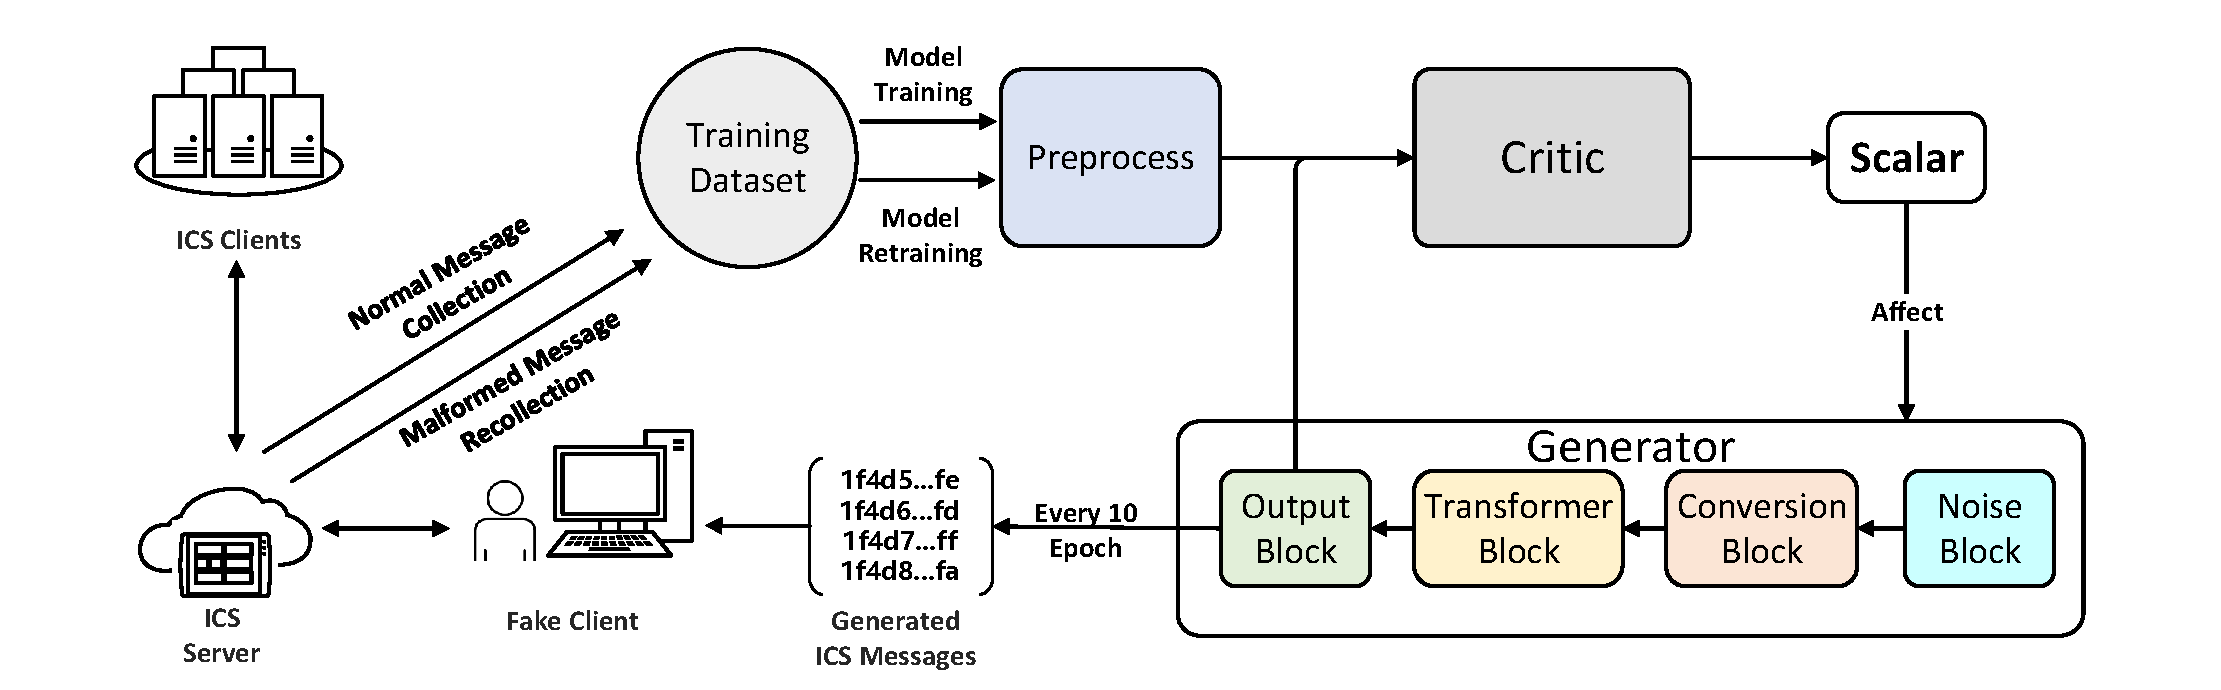
\includegraphics[width=\textwidth]{Figure/FigHexGANFuzzer_model.eps}
	\caption{The framework of HexGANFuzzer}
	\label{FigHexGANFuzzer_model}
\end{figure}

% first acquire a large number of communication data from the ICS to be tested and then
\subsection{Preprocessing of ICP Message Frames}
%diverse test cases, reach high code coverage and
In order to get desirable fuzzing results, data preprocessing is a necessary part. There are two steps in preprocessing: \textbf{Message Frame Clustering} and \textbf{Data Conversion}.

\subsubsection{\textbf{Message Frame Clustering}}
After message frames collection, there are many ICPs' message frames of different lengths. We adopt the Length Clustering method to preprocess the data frames. %It is noted that most message frames with the same length share the same frame type.
First, we gather the data frames which have the same length. %In order not to get too many groups of data frames, 
Groups whose quantity is less than a threshold (e.g. 5000) will be moved to the longer adjacent group, while groups contain more data than the threshold are left unchanged.  %In such a way, there may be message frames with different lengths in one group.
After clustering, the maximum length of message frames of every group will be the standard length and message frames whose length is less than the maximum length will be added special token `u' at the end of them.

\subsubsection{\textbf{Data Conversion}}
The raw data frame of most protocols is hexadecimal, which can not be fed into the model directly. So after clustering, the hexadecimal data frames will be mapped into the digital vectors. The vocabulary we use is as followed:
\begin{equation}
\textit{\textbf{0 1 2 3 4 5 6 7 8 9 a b c d e f u}}
\end{equation}
%The size of the vocabulary is 17, there are ten digits and seven hexadecimal characters according to the hexadecimal message frames and the supplement token `u'.
Based on the vocabulary, message frames $x \in R^{seq\_size \times 1}$ were converted into one hot vector $X \in R^{seq\_size \times 17}$(seq\_size is the maximum length of the current group), and one-hot vectors of real message frame will be the input of the critic.



\subsection{Model Architecture}
\label{sec:model_design} 
As Fig. \ref{FigHexGANFuzzer_model} shows, our model consists of a generator and a critic. 
%, which is the same as a WGAN model
The generator is born to generate the fake message frames and the critic will evaluate the Wasserstein distance. The Wasserstein distance is the minimum cost of transporting mass in converting the data distribution $q$ to the data distribution $p$. During the training, the Wasserstein distance between real message frame distribution and fake message frame distribution will be shortened so that our model grasps specifications of ICPs' grammar.

\subsubsection{\textbf{Generator}}
\begin{figure}[t]   %  插入一栏图片
	\centering 
	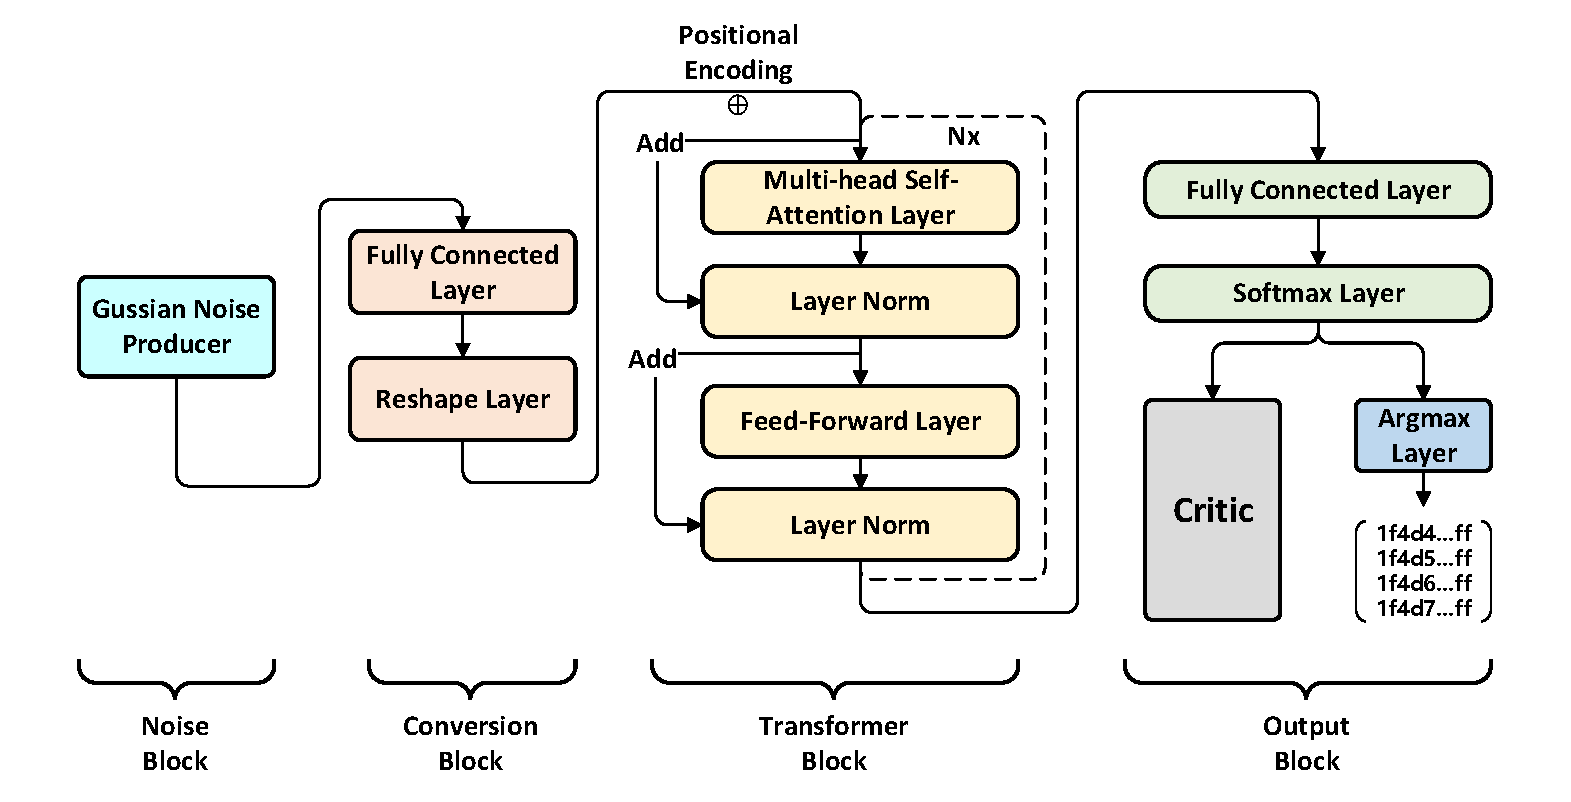
\includegraphics[width=\textwidth]{Figure/FigHexGANFuzzer_Generator.eps}
	\caption{Generator Network}
	\label{FigHexGANFuzzer_Generator}
\end{figure}
%总体描述,分为四个部分,四个部分里面分别是什么,简单介绍作用
The structure of the generator is as followed in Fig. ~\ref{FigHexGANFuzzer_Generator}. 
There are four parts, noise block, conversion block, transformer block, and output block. 

In order to generate different message frame data every time, the noise block will output some random Gaussian distributed noise data $z \in \mathbb{R}^{1 \times zd}$ where $zd$ is the initial dimension of the noise. 
%And it is a common practice to set the noise data to Gaussian distributed noise.

The conversion block contains a fully connected layer and a reshape layer. This block will convert the noise data $z$ into Noise Conversion Representation (NCR) $\tilde{z} \in \mathbb{R}^{ss \times dm}$, where $ss$ is the maximum sequence length of the current group and $dm$ is the number of feature dimensions. NCR is a variant of word embedding with the guarantee of derivative. The package of ICPs is one-dimensional hexadecimal character sequence. 
%For example, the input words of \cite{vaswani2017attention} are converted into word embedding. 
% In our model, 
%The reason we use NCR is that the output of the noise block is a random noise vector, which is hard to get the corresponding word embedding. 
In the NLP tasks, discrete data is usually regarded as the result of continuous sampling from the categorical distribution. If we have to find the word embedding with some tricks, it may cause the whole procedure non-derivable.%, which will make the backpropagation algorithm unavailable. 
The solution of most GAN text generation models is using the one-hot vector to replace the word embedding in the model. But the output of the noise block is a random noise vector, the one-hot vector is hard to featurize representation. %the discrete sequence is represented by two-dimensional vectors including word embedding or one-hot vector for the sake of a better representation of the sequence during the computation in the NLP model.
So in this paper, the discrete sequence is represented by the two-dimensional vector NCR for the sake of a better representation of the sequence. Define the fully connected layer as $f$, noise data $z$ is processed by the reshape operation of $f$ with ReLU activation, and then becomes $\tilde{z} = Reshape(f(z))$ and $ \tilde{z} \in \mathbb{R}^{ss \times {dm}}$. And it is the input of the transformer block.  %, but it is fake. %NCR maps the one-dimension noise vector to high dimensional space information. Compared with the one-hot vector, NCR can cover more information of high dimension space.

The transformer block is applied as a feature extractor. It contains a positional encoding layer and a sub-block. The sub-block is the same as the encoder part of the Transformer \cite{vaswani2017attention}. It is formed by a multi-head self-attention layer and a feed-forward layer. Besides, there is a residual connection around each of the two layers, followed by layer normalization. Compared with the commonly used Recurrent Neural Network (RNN), the transformer block is better in semantic feature extraction and long-range feature extraction. Moreover, the self-attention layer in the transformer block supports parallel training, which can accelerate the training process. %And the input and output of the transformer block are the same, so this part can repeat as many times as we want. %the conversion block and the transformer

The output block includes a fully connected layer and a softmax layer. After the output block, the generator will not output the message frame data directly, instead, it outputs a probability vector $\tilde{x} \in \mathbb{R}^{ss \times vs}$, Where ${vs}$ is the size of vocabulary. %, which is $17$ in this paper 
The probability vector is an intermediate result which is used to feed the critic. To obtain the generated message frame for fuzzing, the probability vector will be applied $argmax$ function and be translated into hexadecimal characters according to the vocabulary mentioned before. The loss function of the generator is:
\begin{equation}
L_{g} = - \mathop{\mathbb{E}}\limits_{\tilde{x}\sim\mathbb{P}_{g}}\left [ D(\tilde{x}) \right ] 
\end{equation}
where D is a 1-Lipschitz function, $\tilde{x} \in \mathbb{R}^{ss \times vs}$ is the output of the generator, $\mathbb{P}_g$ is the model distribution implicitly defined by $\tilde{x}=G(z)$, and $z$ is the noise data.

\subsubsection{\textbf{Critic}}

The discriminant model looks like the discriminator in common GAN models, but it is not a classifier. So we call it critic here, following WGAN \cite{arjovsky2017wasserstein}. The structure of the critic is shown in Fig. \ref{FigHexGANFuzzer_Critic}. The critic includes five conv-1d layers, five self-attention layers, and one fully connected layer. For the critic, there are two types of inputs: the one-hot vector from the real message frames, and the output of the generator which represents the fake message frames. 
The second dimension of the output of the generator indicates the probability of each character in the vocabulary, and the one-hot vector can be regarded as a special case of it. %that is, the probability of one word is 1 and the probability of other words is 0. 

\begin{figure}[htbp]   %  插入一栏图片
	\centering 
	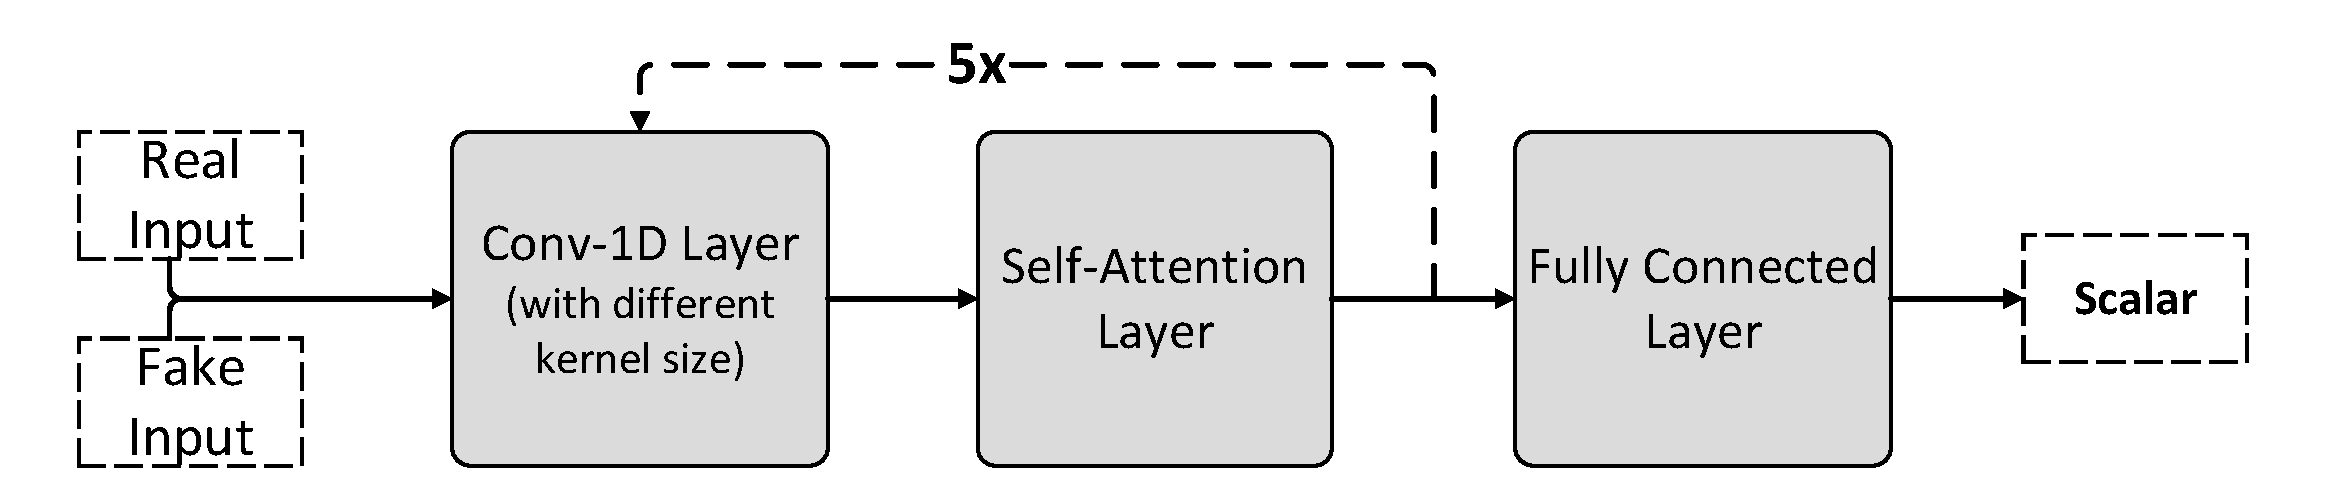
\includegraphics[width=\textwidth]{Figure/FigHexGANFuzzer_Critic.eps}
	\caption{Critic Network}
	\label{FigHexGANFuzzer_Critic}
\end{figure}

It is noted that the first conv-1d layer changes the second dimension of inputs from the probability of word to the feature representation, which is the same as the dimension of NCR. And other conv-1d layers keep the second dimension as $dm$. Every conv-1d layer followed by a self-attention layer but the kernel size of conv-1d is not the same. The kernel size of $i$th conv-1d layer $ks_i = i$ where $i \in \{1,2,3,4,5\}$. 

Protocols have message headers, which specify the content of the message body in the message frame. More simply, the front part of the message frame affects the back part. It is hard to distinguish the boundary of two parts without the knowledge of the protocol grammar. If the model has learned which part is the message header, it can pay more attention to the message header part.
Due to different protocols have different lengths of the message header, the conv-1d layer with different kernel size can capture the information better.

%self-attention layers can capture how flags in the message header affect the part of the message body.
%With the boundary information leaned by conv-1d layers, self-attention layers will pay more attention to the correlation between the content in the message header and body. 

As for the content in the message header, several flags in the message header affect different parts of the content in the message body. Self-attention layers consider the attention weight of every position of the input and is good at learning long-range dependencies. With the boundary information leaned by conv-1d layers, self-attention layers can capture how flags in the message header affect the part of the message body. After repeated self-attention and conv-1d layers five times, the fully connected layer will output a scalar score. The loss of the critic is:
\begin{equation}
L_{c} = \mathop{\mathbb{E}}\limits_{\tilde{x}\sim\mathbb{P}_{g}}\left [ D(\tilde{x}) \right ] 
- \mathop{\mathbb{E}}\limits_{x\sim\mathbb{P}_{r}}\left [ D(x) \right ] 
+ \lambda\mathop{\mathbb{E}}\limits_{\hat{x}\sim\mathbb{P}_{\hat{x}}}\left [ ( \left \| \triangledown_{\hat{x}}D( \hat{x}) \right \|_{2} - 1 )^{2} \right ]
\end{equation}
where $\mathbb{P}_{\tilde{x}}$ defines sampling uniformly along straight lines between pairs of points sampled from the real data distribution $\mathbb{P}_{r}$ and the generator distribution $\mathbb{P}_{g}$. 
In order to satisfy the 1-Lipschitz constraint, the solution of the WGAN-GP model is adopted. 
We use the gradient penalty instead of the weight clipping to enforce the 1-Lipschitz constraint, which leads to a more stable training process.% and the model is easier to train.

\subsubsection{\textbf{Training strategy}}
%Once the model design is completed, we begin to train our model. Under normal circumstances, the training of the GAN is adversarial, which means the generator and discriminator (critic) should be on the same level. If the imbalance is too serious, another one will learn nothing. And this is the reason why the GAN model is difficult to train and the training is unstable.
Due to the properties of the Wasserstein distance, we train the critic better to narrow the Wasserstein distance between fake message frame distribution and real message frame distribution. %, which is the process of improving generator. 
In every epoch, we train generator once and then train the critic $c\_iters$ ($5$ in our model) times. %Adam Optimizer was used both in the generator and the critic. 
In order to judge the convergence of the model, the following equation approximately indicates the value of the Wasserstein distance. If the value of the equation trends to be stable, we consider the model is convergent.
\begin{equation}
W\_distance = 
\mathop{\mathbb{E}}\limits_{x\sim\mathbb{P}_{r}}\left [ D(x) \right ] 
- \mathop{\mathbb{E}}\limits_{\tilde{x}\sim\mathbb{P}_{g}}\left [ D(\tilde{x}) \right ] 
\end{equation}
%Though the model wants to generate the fake message frames that share high similarity to the real message frames, the ulmate goal is to achieve effective fuzzing results and identify as many bugs as possible. In order to obtain the desired results, there should be some differences between the real data and the fake data. So we not only save the final version of the model, which is convergent, but also the intermediate generator model. The model was saved every 10 training epoch deliberately. In such a training strategy, the goal of the high code coverage and deeper testing depth can be achieved.
The model is saved every 10 training epoch deliberately to achieve the goal of the high code coverage and deeper testing depth. Test cases that cause target anomalies will be recollected and put into the training dataset again. Data augmentation and value mutation operation are applied to these data before putting it into the dataset. We assume that retraining the model with these data can improve the capability of the model to discover vulnerabilities.



\section{Experiment and Result Analysis}
In this section, MQTT and Modbus are chosen as our test targets from a variety of ICPs in the experiment. We generate a lot of test cases using the generative model. Then the generated data is used to stress test the target and trigger anomalies of the ICP. Finally,  according to the anomalies triggered, vulnerabilities in the anomalies are submitted for the improvement of the ICP after analysis to find the reason for the target anomalies. We evaluate the effectiveness of the proposed method by experimentation. 

\subsection{Environment construction of MQTT and Modbus}
To show the effectiveness and efficiency of our framework, we apply it to test MQTT, one of the mainstream ICPs. To indicate the versatility of our method, another ICP, Modbus, is also used to test.

\subsubsection{MQTT}
MQTT (Message Queuing Telemetry Transport) protocol is an application layer ICP based on publication and subscription under the ISO (International Organization for Standardization) standard and works on the TCP/IP protocol cluster. It is simple to implement, provides the transmission data with the quality of service, has the characteristics of lightweight, high bandwidth utilization efficiency, data independence and so on. The message format of MQTT is illustrated in Fig. \ref{FigMQTTFormat}.  

\begin{figure}[htbp]   %  插入一栏图片
	\centering 
	\includegraphics[width=3.5in]{FigMQTTFormat.pdf}
	\caption{Message format of MQTT}
	\label{FigMQTTFormat}
\end{figure}

In the experiment, we utilize Mosquitto v1.5.8 \cite{light2017mosquitto} as the open-source message broker of message push ICP MQTT v3.1 and  Paho-MQTT v1.0.2 \cite{light2017mosquitto} as the MQTT client. 

\subsubsection{Modbust-TCP}
There are many variants of Modbus, including Modbus-TCP, Modbus-UDP and so on. We choose Modbus-TCP as another fuzzing ICP in this study. It uses master-slave communication mode, in which the master communicates with the slave by sending and receiving data frames \cite{swales1999open}. 

\subsection{Evaluation Setup}
\subsubsection{Experimental Environment}
Tensorflow, one of the popular deep learning framework in the industrial community, is adopted to implement the model architecture. To improve the training efficiency, we train the model on a machine with 8 processors (Intel(R) Core (TM) i7-6700K CPU@4.00GHz)  16.0GB memory (RAM) Nvidia GeForce GTX 1080 Ti (11GB) and 64-bit ubuntu16.04, x64-based processor. When launching an attack, the simulators run on another machine with 4 processors (Intel (R) Core (TM) i5-5300U CPU@2.30GHz) 16.00GB memory (RAM) and 64-bit Microsoft Windows 10 Professional Operating System, x64-based processor.

\subsubsection{Model Training Setting}
As for the parameter setting, we initialize all weights from zero-centered Normal distribution with a standard deviation of 0.2, which can increase diversity to a certain extent. The mini-batch size is set to 32 in all models based on a large amount of training data. The $keep\_prob$ hyperparameter of dropout is set to 0.7. The learning rate of G and D is set to 0.0001 and 0.0004 in the Adam optimizer. As to the checkpoint in the generative model, the interval of model saving frequency is set to 10. We train the models for 100 epochs and save the generator model for every 10 epochs to get plentiful test cases.

\subsection{Fuzz Testing The Target ICP}
With the trained model, we generate test cases, input the system under test, and implement the fuzzy test process according to the standard fuzzy test process. In the process of inputting test cases into ICSs under test, we monitor the system in real time. If anomalies occur in the process, such as the output clobber problems and interface crash, we record and restart the test process at the current point. At the end of the entire test, we analyze the causes of antecedent anomalies and the logs of server systems to find the running status of potential vulnerabilities.

\begin{figure*}[htbp] 		 %  插入双栏图片
	\centering
	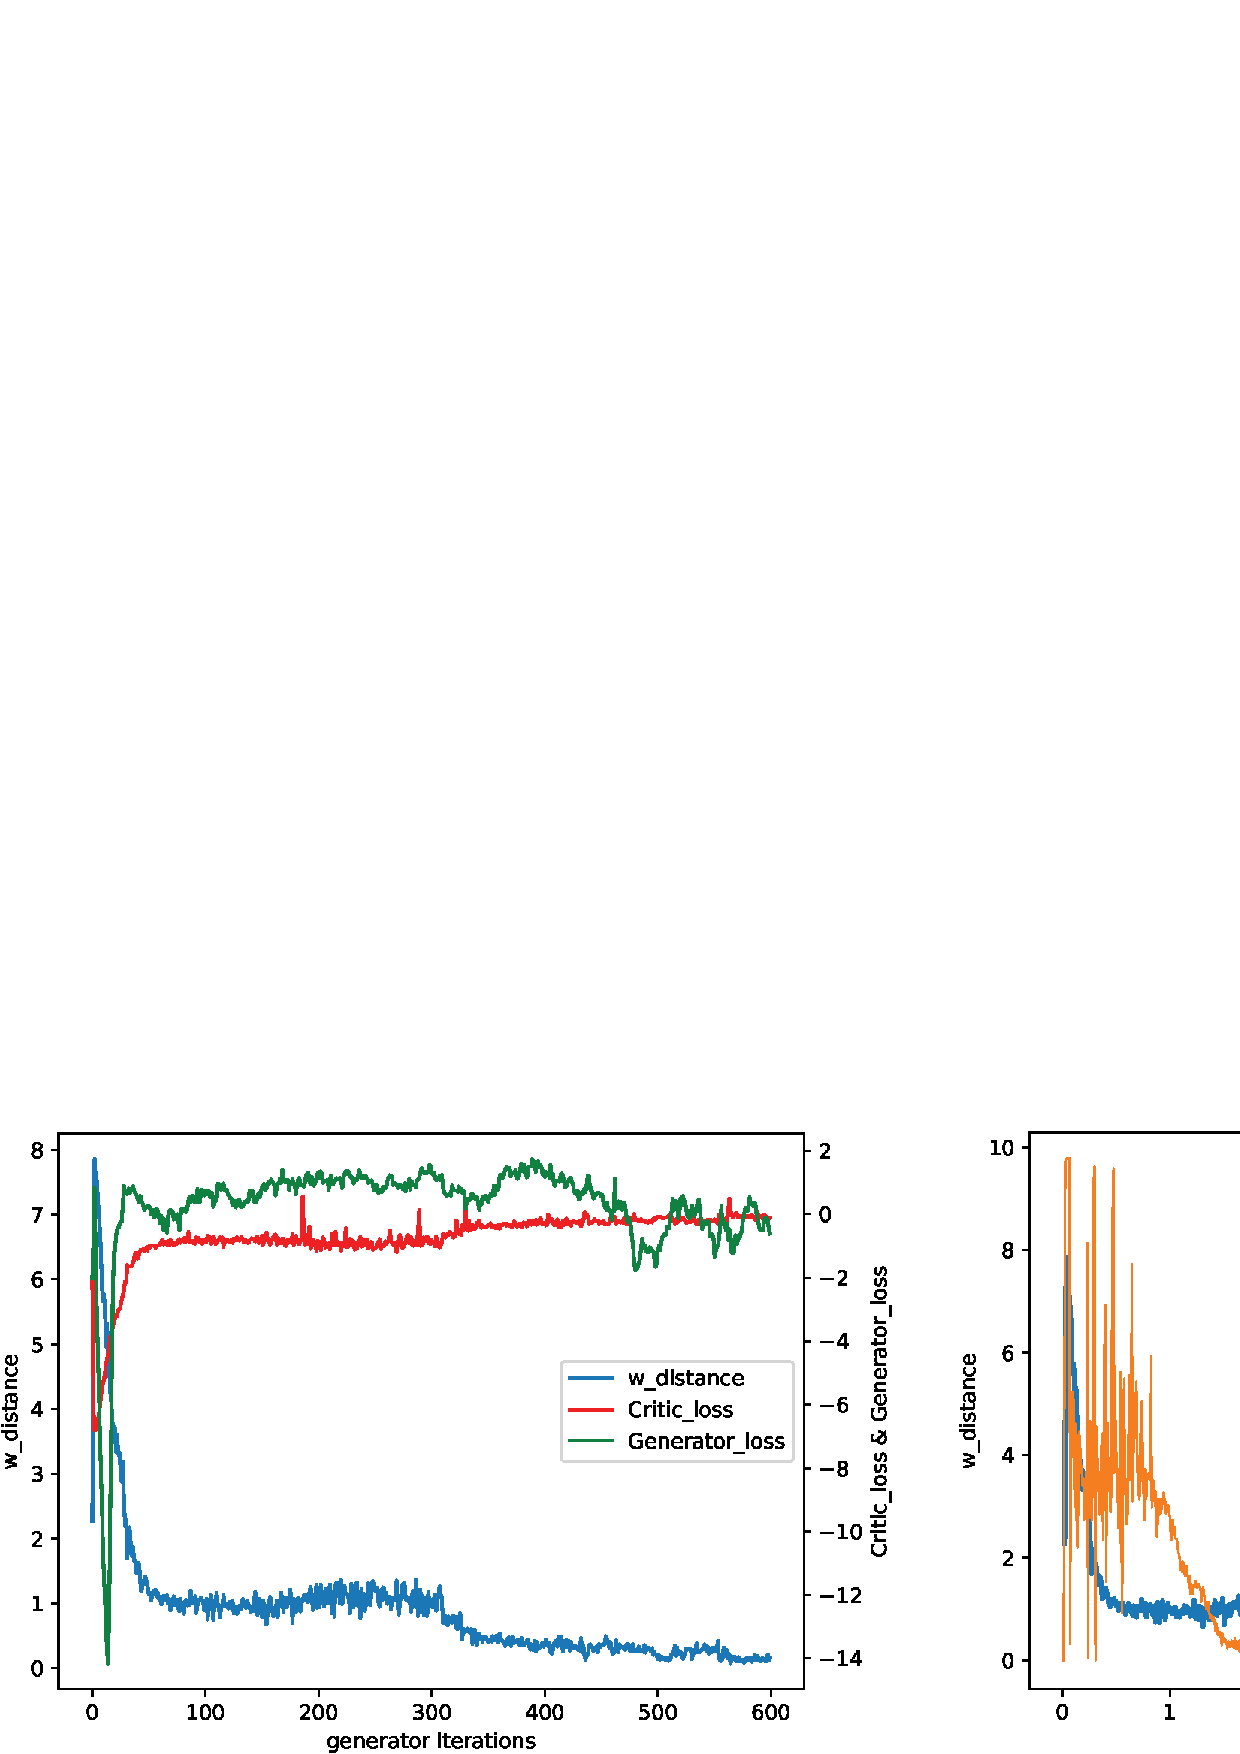
\includegraphics[width=5.5in]{FigModelW-distance.pdf}
	\caption{Dataset(500,000 test cases) W-distance over generator iterations (left) or wall-clock time (right) for SAGANFuzzer}
	\label{FigModelW-distance}
\end{figure*} 

\subsubsection{Training Data}
Training data in deep learning significantly influence model training. In the experiment, training data about the two industrial control protocols is collected separately. 

\begin{figure}[htbp]   %  插入一栏图片
	\centering 
	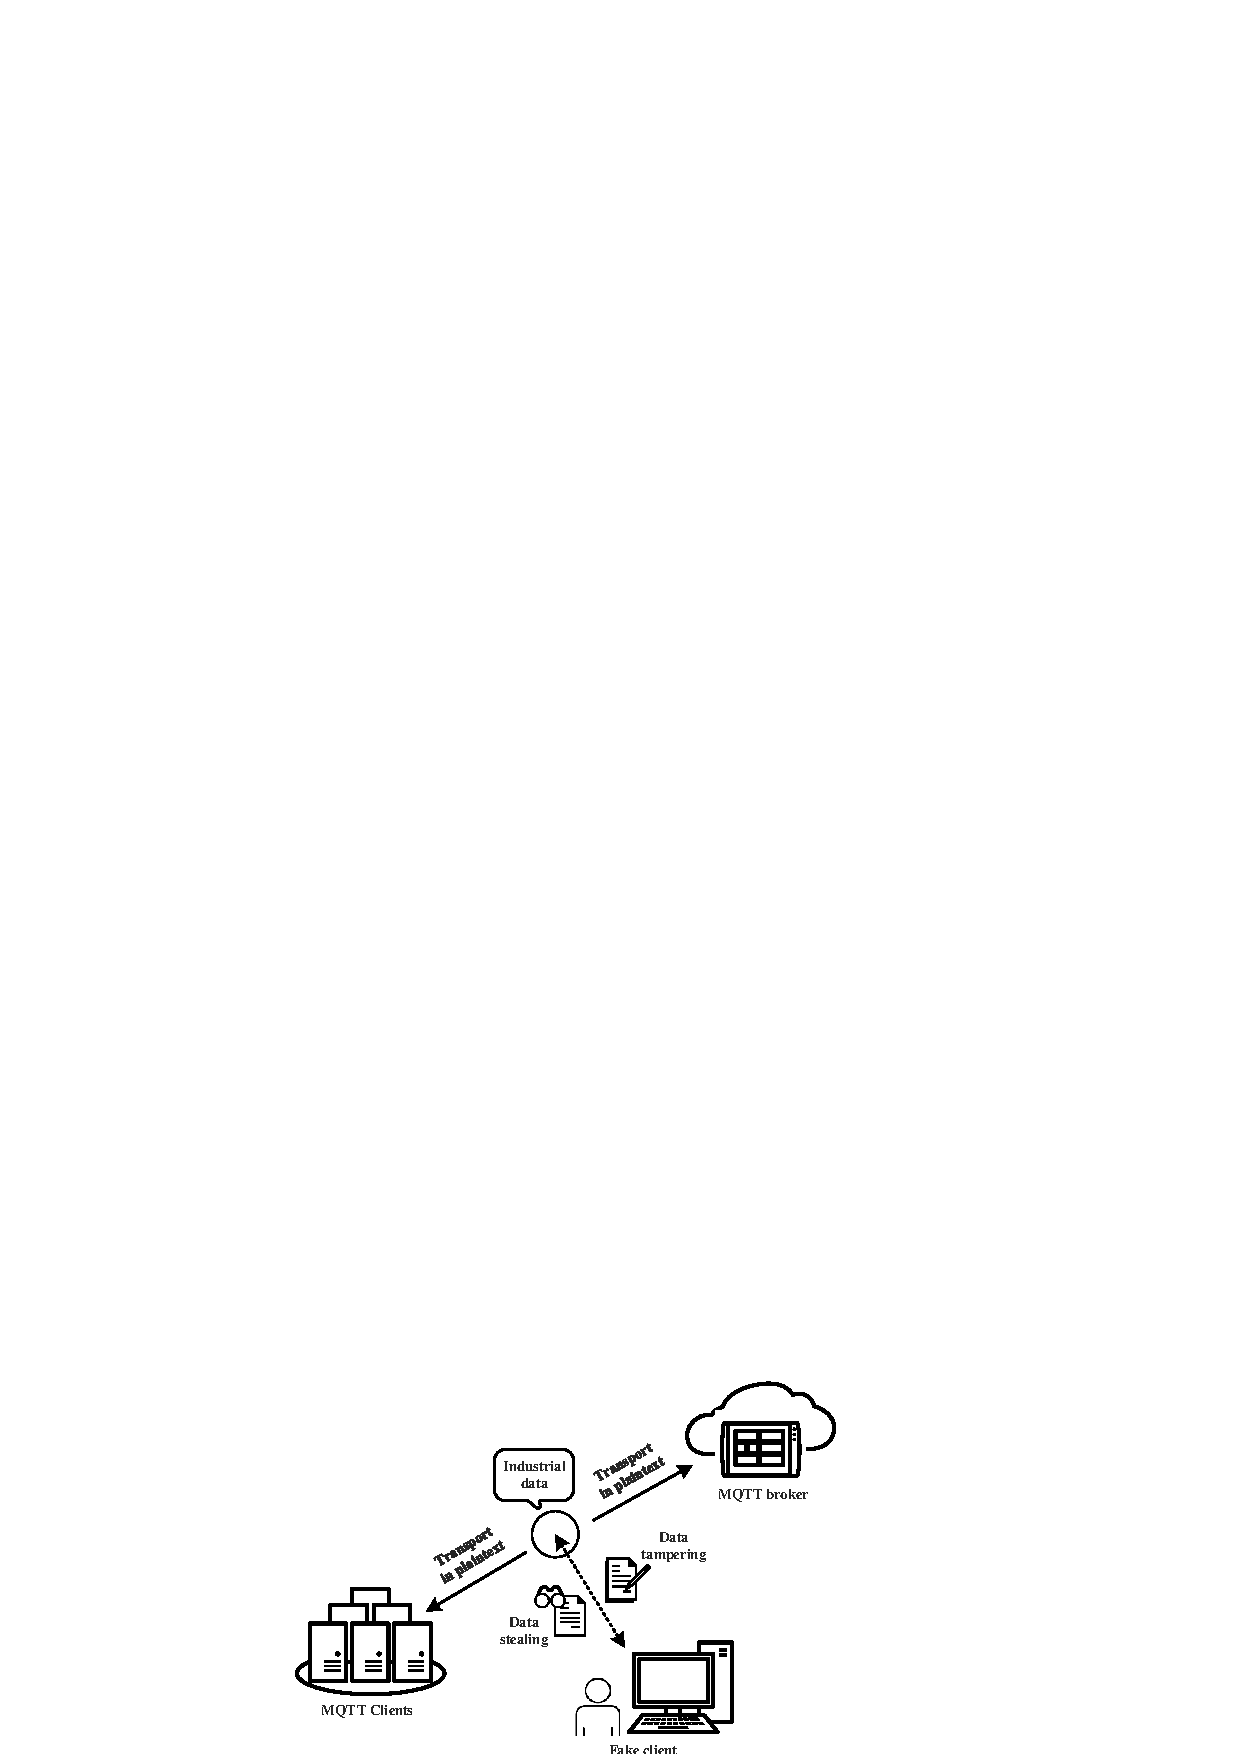
\includegraphics[width=3in]{FigMQTTEnvironment.pdf}
	\caption{MQTT enviroment}
	\label{FigMQTTEnvironment}
\end{figure}

\quad \textit{\textbf{a. MQTT.}}
In order to capture the MQTT communication data, an MQTT network environment based ICS is prepared as illustrated in Fig. \ref{FigMQTTEnvironment}. Wireshark \cite{orebaugh2006wireshark} is applied to grab packets during communication. These grabbed frames serve as the training data for the SAGANFuzzer framework. 
After fetching the connection information between the legal clients and the MQTT broker, we construct a disguised MQTT client to send the same connection information to connect to the broker in the IoT network with no authentication security measures. The disguised MQTT client launches the attack by sending fake MQTT messages which are generated by fuzzy test models. 

\quad \textit{\textbf{b. Modbus-TCP.}}
Pymodbus \cite{collins2013pymodbus}, a python package that implements the Modbus protocol, is used to generate the training data frames. Enough different types of data frames can be generated quickly via Pymodbus, which is practical and convenient. In the experiment, a Modbus-TCP implementation, Modbus RSSim v8.20, is applied as the fuzzing targets. The generated test cases are sent to the Modbus-TCP implementation by a python script over sockets to test the effects in simulated applications.


\subsubsection{Model Training}

One advantage of our method over weight clipping is largely overcoming the problem of unstable training of GANs, such as non-convergence, vanishing gradient and mode collapse. We design our model architecture based on these architectural constraints and improve training speed and sample quality. To demonstrate this, we train SAGANFuzzer with W-distance and gradient penalty on a dataset with 500,000 test cases and plot W-distance and losses of the generator and the discriminator of training in Figure \ref{FigModelW-distance}.



Following the setting in the subsection Model Training Setting, we train one model with the same optimizer (Adam) and learning rate as WGAN with weight clipping. The results also represent that our method converges faster and is more stable at convergence.

\subsubsection{Logging and Evaluation}
Logging is the basis for further analysis of model performance and fuzzing effectiveness. By analyzing logs of the communication process is an effective method to find ICPs’ anomalies. Some vulnerabilities may be manifested according to the obvious abnormal behavior of the system, and some behaviors need to be further analyzed. Based on the statistical analysis of the log file, we evaluate experimental results. Furthermore, we artificially analyze specific anomalies to get more details. Test data that causes target anomalies will be recollected and put into the training data set again. Data augmentation and value mutation operation will be applied to these data before putting it into the retraining data set. The retrained model with these mutated data can improve the capability of the model to detect vulnerabilities.

\subsection{Result Analysis}
In this part, we show the experimental results in three aspects. We first present some special anomalies that occurred in fuzzing the MQTT implementations. Then we reveal statistical results and their analysis. Lastly, to show the methodology’s protocol independence in ICP’s fuzz testing, the result of testing Modbus-TCP is presented.

\subsubsection{Statistical Analysis And Results}
The widely used General Purpose Fuzzer(GPF) \cite{demott2007revolutionizing}, CNN-1D model, LSTM-based seq2seq model, and WGAN-based model are chosen as fuzzers in the control group in this study. After fuzzers in the experimental group and control group are fully trained, fuzz testing is conducted by sending a total of 500,000 generated test cases to MQTT implementations through the TCP/1883 port.

According to the three aforementioned evaluation metrics, the effectiveness and efficiency of our fuzzing framework SAGANFuzzer and fuzzers in the control group are evaluated and represented graphically. Details are as follows.  

\begin{table*}[]
	\centering
	\caption{Performance Metrics Comparison}
	\label{F-measure}
	\renewcommand{\arraystretch}{1.35}
	\begin{tabular}{ m{70pt}<{\centering} |m{70pt}<{\centering}|m{40pt}<{\centering}|m{60pt}<{\centering}|m{40pt}<{\centering}|m{40pt}<{\centering}|m{40pt}<{\centering}}
		\toprule
		\textbf{Dataset
			(number of training cases)} & \textbf{Methods}          & \textbf{Year} & \textbf{F-measure} & \textbf{SE}     & \textbf{SP}     & \textbf{AC}     \\ \midrule
		& GPF              & 2007 & --         & 0.5252 & 0.5798 & 0.6474 \\ \cmidrule(l){2-7} 
		& CNN-1D model     & 2014 & 0.6701    & 0.8437 & 0.9743 & 0.8626 \\ \cmidrule(l){2-7} 
		10,000  & LSTM-based model & 2018 & 0.6300    & 0.8563 & 0.9007 & 0.8254 \\ \cmidrule(l){2-7} 
		& WGAN-based model & 2019 & 0.7960    & 0.7696 & 0.9115 & 0.8165 \\ \cmidrule(l){2-7} 
		& SAGANFuzzer      & 2020 & 0.8208    & 0.8274 & 0.9775 & 0.8608 \\ \midrule
		& GPF              & 2007 & --         & 0.5720 & 0.5730 & 0.6510 \\ \cmidrule(l){2-7} 
		& CNN-1D model     & 2014 & 0.8373    & 0.8670 & 0.9842 & 0.8690 \\ \cmidrule(l){2-7} 
		500,000 & LSTM-based model & 2018 & 0.8588    & 0.8203 & 0.9856 & 0.8700 \\ \cmidrule(l){2-7} 
		& WGAN-based model & 2019 & 0.8396    & 0.8108 & 0.9871 & 0.8906 \\ \cmidrule(l){2-7} 
		& SAGANFuzzer      & 2020 & 0.8502    & 0.8538 & 0.9878 & 0.9271 \\ \bottomrule
	\end{tabular}
\end{table*}

\quad \textit{\textbf{a. F-measure.}} Table \ref{F-measure} shows the accuracy of each method in generating legitimate test cases on a dataset of 10,000 and 500,000 training data. It can be observed from the table that the algorithm in this paper has Higher scores of Sensitivity, Accuracy, F-measure than CNN-1D model, LSTM-based seq2seq model and WGAN-based model in datasets of different sizes. Although the Sensitivity of the CNN-1D model and LSTM-based seq2seq model is higher than that of the method in this paper, the types of test cases generated are relatively single, and the algorithm in this paper has the highest F-measure. For the dataset of 10,000 training data, the F-measure of generating legitimate test cases reaches 82.08\%, which is 2.48\% higher than the WGAN-based model, and the Sensitivity of this method is 5.78\% higher than that of the WGAN-based model. On the dataset of 500,000 training data, our method is 1.06\% higher in F-measure and 4.30\% higher in Sensitivity than the WGAN-based model. 

Therefore, we can draw a conclusion from the evaluation metrics of the performance of machine learning models in the table: in terms of datasets with different data sizes, the model in this paper is superior to other fuzzy test case methods in each evaluation metric of generating legitimate test cases.


\quad \textit{\textbf{b. EVD.}}
In order to map the EVD values of each model to a relatively small scope for diagrammatic comparison, we normalize all EVD values under the same iteration through Z-score standardization. The experimental results of EVD are shown in Fig. \ref{FIGURE_EVD}. Due to not involving a continuously learning process, the performance of GPF has a downward trend on the targets when compared to the other four fuzzing models based on depth learning. From the perspective of the five models, the performance of the EVD indicators is: GPF $\textless$ CNN-1D model $\approx$ LSTM-based model $\textless$ GAN-based model $\textless$ SAGANFuzzer. 

\begin{figure}[htbp]
	\centering
	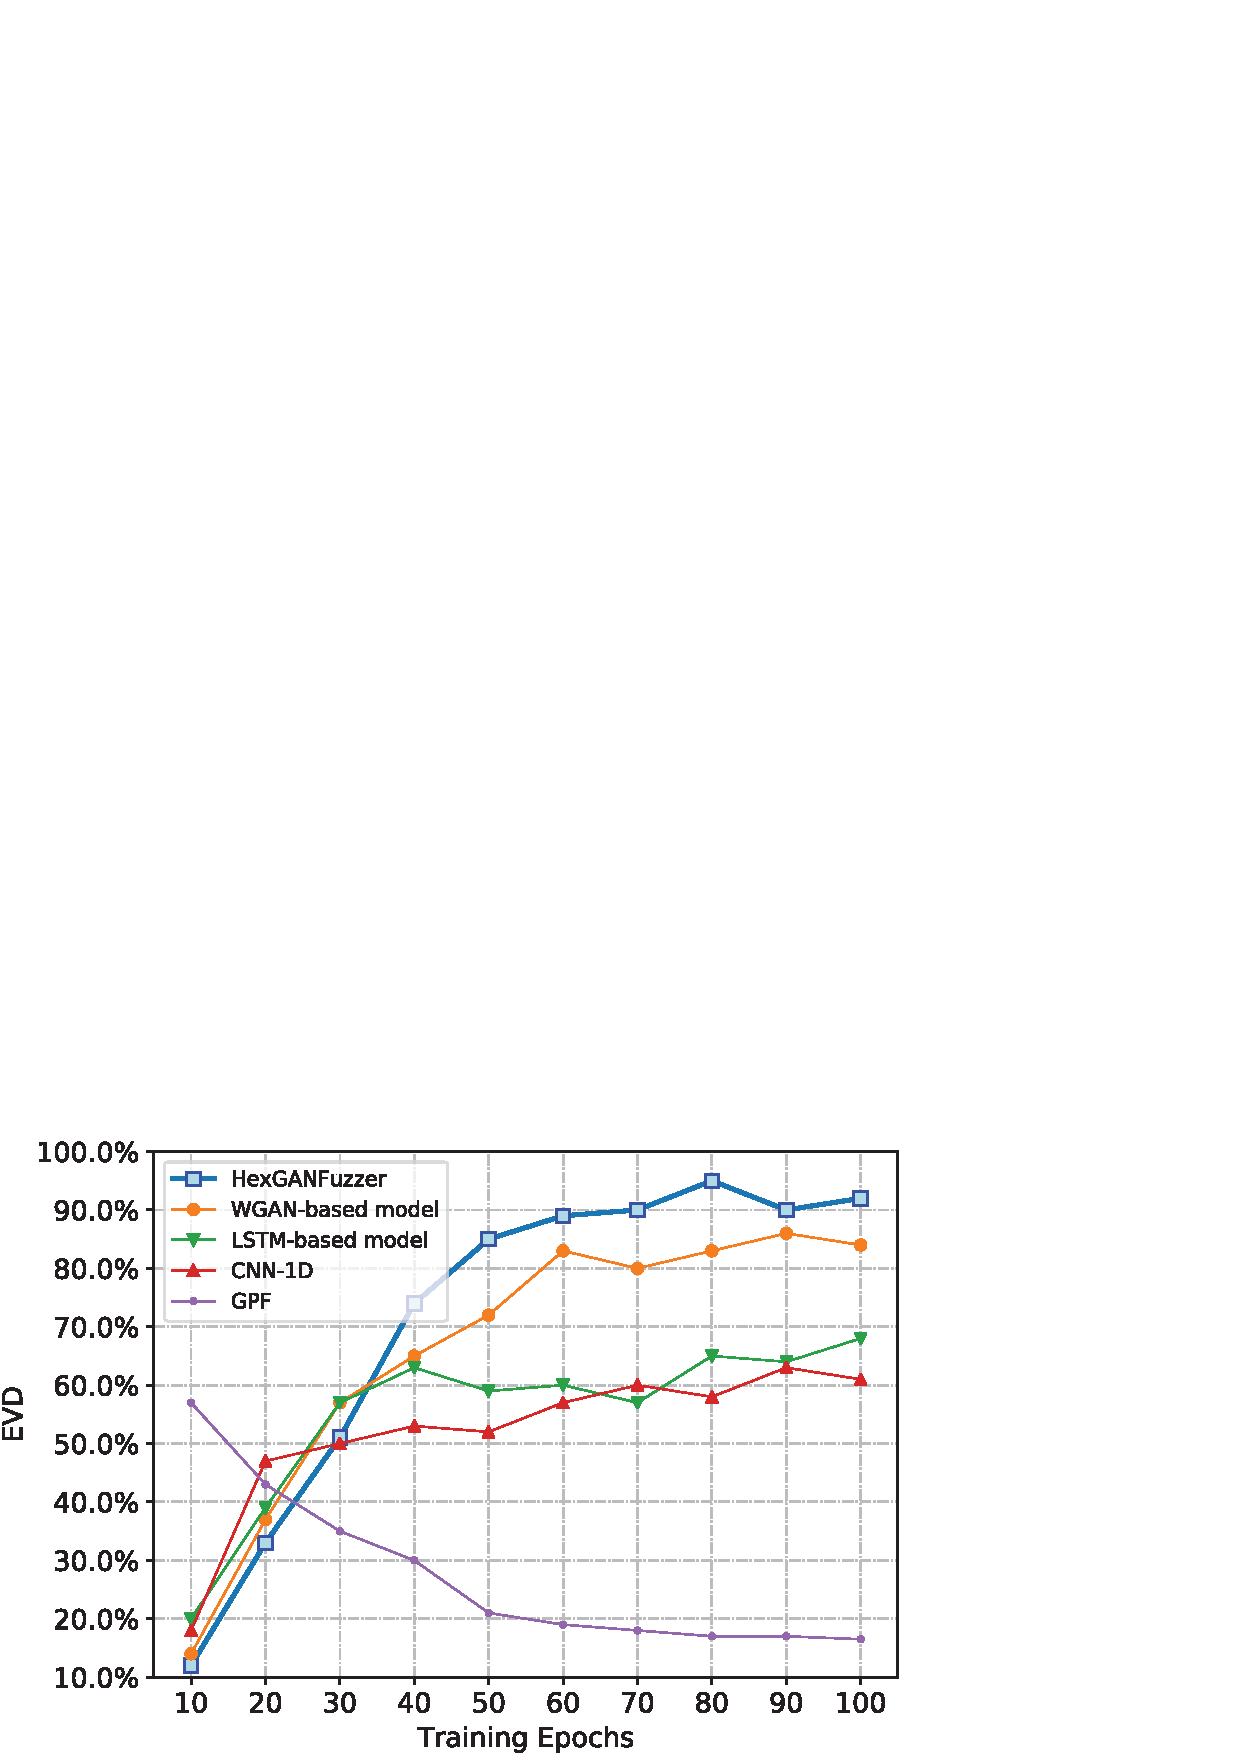
\includegraphics[width=3.36in]{FIGURE_EVD.jpg}
	\caption{EVD changes with the training epochs}
	\label{FIGURE_EVD}
\end{figure}
%generative adversarial
After training more than 30 epochs, the EVD rates of deep learning algorithms obviously exceed the GPF algorithm. With the rising trends of rates slow down significantly after 50 epochs, the average EVD rates of CNN-1D model and LSTM-based model are 60\% to 70\% compared with 75\% to 90\% of generative adversarial algorithms, which may be caused by the inability to learn a hierarchy of representations of the data effectively. Due to the unsupervised characteristic of generative adversarial algorithms, it may result in generating a large number of malformed protocol message sequences, leading to normal throwing which may cause EVD can not be further promoted. But for the generative adversarial algorithms from 50 to 100 epochs, the average EVD rate of SAGANFuzzer is approximately 8\% higher than the WGAN-based model, which indirectly indicates that SAGANFuzzer is more applicable to test cases generation for ICPs. It's worth going into detail that our trained model can effectively detect kinds of anomalies as presented in Table \ref{Triggered_Anomalies_SAGANFuzzer} with the gradient penalty, which shows we are likely to achieve the higher code coverage and the stronger ability of our model has to detect anomalies.
%Usually, the richer the data type, the higher code coverage we are likely to achieve, and the stronger ability a model has to detect anomalies.
\begin{table}[htbp]
	\caption{Triggered Anomalies and Triggered Frequency of SAGANFuzzer}
	\label{Triggered_Anomalies_SAGANFuzzer}
	\centering
	%
	\begin{tabular}{m{100pt}<{\centering}  m{40pt}<{\centering} m{50pt}<{\centering} }
		\toprule
		\bfseries Triggered Anomalies &  \bfseries Frequency (Times) & \bfseries ATITA (Mins)\\
		\midrule
		Using abnormal function code & 104 & 5.78\\
		Automatically closes window & 53 &10.64\\
		Data length unmatched & 121 & 4.52\\
		Abnormal address & 23 &13.26\\
		Integer overflow & 7 & 114.49 \\
		Broker memory overflow & 2 & 285.05 \\
		\bottomrule
	\end{tabular}
\end{table}

where Frequency represents the number at which the specified type of anomalies is triggered by the models during test time and average time interval of triggered anomalies (ATITA) is the quotient of the number of triggered anomalies and test time.

\quad \textit{\textbf{c. EFVD.}}
There is a huge difference in the training time of different GPF and the time of anomalies triggered by GPF is constant under different iterations, so it is not discussed in this part. The normalization of EVD is applied to EFVD, too. The testing depth has increased as illustrated in Fig. \ref{FIGURE_EVD} at the expense of reducing the code coverage of fuzz testing. But what makes a difference, rather, is that high test efficiency is maintained on the premise of attaining high EVD rates. The variation trend of EFVD of different deep learning based models is presented in Fig. \ref{FIGURE_EFVD}. It can be seen from the figure that when doing less training epochs, models with relatively short training time can achieve higher EFVD scores. And with the deepening of training, TAT values of different models become more and more different, so models with higher potential efficiency of vulnerability detection will get higher EFVD scores. Looking at the overall trend, the average EFVD score of our model is 19.45\% higher than that in the CNN-1D model, 15.14\% higher than the LSTM-based model and 5.26\% higher than the WGAN-based model. And the fluctuation of our model is relatively small, which indicates that our model can maintain relatively stable efficiency on the basis of balancing TT and TAT.

%When the training epochs is 10, the TT of the four deep learning based models maintains the best. After training, some message categories are generally lost, as presented in Fig. \ref{FIGURE_EFVD}.。

%A total of 13 categories of Modbus data frames are prepared in the raw data. 

%When the training epochs is 10, the diversity of the three deep learning based models maintains the best. 

%After training, some message categories are generally lost.

%BLSTM-DCNNFuzz and LSTM-based model have a good performance on maintaining basically the test case diversity, which illustrates the two models can learn the time-step dimension of protocol messages. And owing to the BLSTM model containing two sub-networks for the forward and backward sequence context respectively, it is able for the BLSTM-DCNNFuzz to exploit information from both the past and the future, which performs better than LSTM-based model. 

\begin{figure}[htbp]
	\centering
	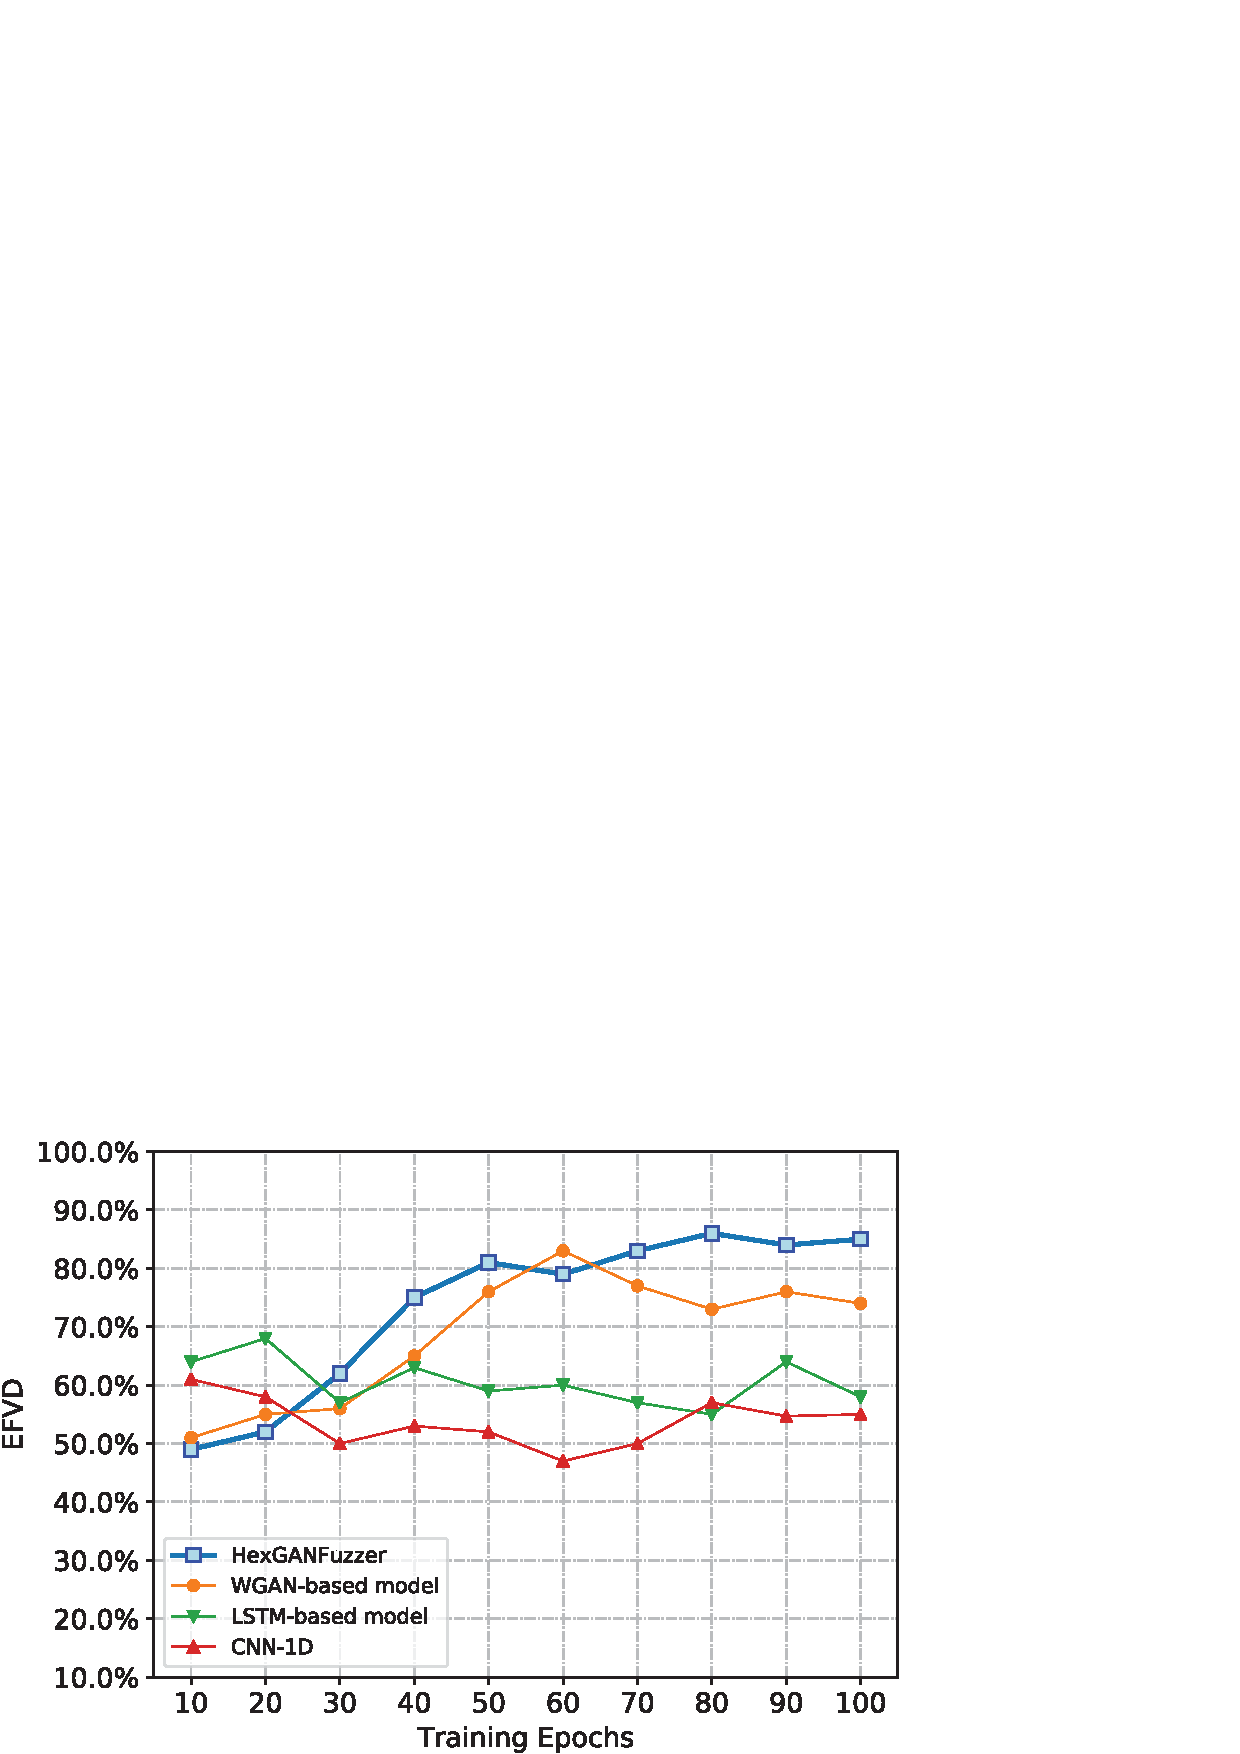
\includegraphics[width=3.3in]{FIGURE_EFVD.jpg}
	\caption{EFVD changes with the training epochs}
	\label{FIGURE_EFVD}
\end{figure}

%\subsubsection{Potential Vulnerabilities Found}

\subsubsection{Applying The Method to Modbus-TCP}
As shown in Table \ref{table_MQTT}, we detect these potential vulnerabilities, including slave crash, station off-line, working counter attack, using abnormal function code and so on, in Modbus-TCP via the new trained SAGANFuzzer. In the experiment, we send the generated data messages $S_i$ to the slave stations and record the corresponding received message $R_i$. Massive message pairs $<S_i, R_i>$ are obtained. According to the abnormal protocol characterization above, we analyze and compare the specified field values and obtained the following statistical results. Experiments on the Modbus-TCP protocol prove that our method has great versatility.% {350pt}{lcc}

\begin{table}[htbp]
	\caption{Potential Vulnerabilities and  in Modbus-TCP}
	\label{table_MQTT}
	\centering
	\begin{tabular} {p{100pt}<{\centering} p{40pt}<{\centering} p{50pt}<{\centering}}
		\toprule
		\makecell[tl]{\bfseries Triggered Anomalies} &  {\bfseries NTA} & {\bfseries ATITA (Mins)} \\
		\midrule
		\makecell[tl]{Slave crash}  & {29 times} & 21.11 \\
		\makecell[tl]{Station ID xx off-line} & {164 times} & 0.79 \\
		\makecell[tl]{Working counter attack}   & {14 times } &  28.13\\
		\makecell[tl]{Using abnormal function code}  & {207 times} & 0.52 \\
		\makecell[tl]{Automatically closes window}  & {13 times} & 28.47 \\
		\makecell[tl]{Data length unmatched}  & {190 times} & 0.63\\
		\makecell[tl]{Debugger memory overflow}  & {4 times} & 41.85 \\
		\makecell[tl]{Unknown attack}  & {197 times} & 0.59 \\
		\bottomrule
	\end{tabular}
\end{table}
where number of Triggered anomalies(NTA) represents the total number of anomalies triggered by the models during test time.

%On the one hand, on account of directly calculating the relationship between any two hexadecimal characters to obtain the global geometric features in sequences, self-attention makes the extracted features more accurate in one step. On the other hand, the number of layers is strictly limited in the case of ensuring the accuracy to reduce the size of the model. 
\section{Conclusions and Future works}

%Fuzzy test based on deep adversarial learning is of great practical significance to the security verification of ICP. 
This paper applies deep adversarial learning from a self-attention perspective to generate fake but plausible fuzzing protocol messages of ICPs. We combine Wasserstein distance with self-attention to the model, making the model training more stable and computing hidden relationship between any two hexadecimal characters in parallel for all the input and output. And gradient penalty is applied to enforce the 1-Lipschitz constraint, which maintains the diversity of the generated data. The performance of our method is verified on datasets of different data sizes: the accuracy of the datasets containing 10,000 and 500,000 training data are 86.08\% and 92.71\% respectively, and F-measure are 82.08\% and 85.02\% respectively.

Our work motivates many avenues for future research, such as: GAN Compression \cite{li2020gan}, online learning with being deployed in embedded devices and anti-random strategies to improve the probability of anomalies triggering.
% Considering the current situation, we intend to perform the study in the following aspects in future studies. First, GAN Compression \cite{li2020gan} is a good way to keep the model more lightweight. And it is a promising application scenario that the lightweight model with online learning capabilities is deployed in embedded devices, which can learn protocol specifications or message formats of different protocols automatically. Second, a series of anti-random strategies after model training to improve the probability of anomalies triggering. Finally, we plan to apply the improved WGAN for more complex unsupervised learning NLP tasks including stateful protocols and non-stateful protocols. 




\nocite{*}
\bibliographystyle{IEEEtran}
\bibliography{Reference}

\end{document}
